%*******10********20********30********40********50********60********70********80

% For all chapters, use the newdefined chap{} instead of chapter{}
% This will make the text at the top-left of the page be the same as the chapter

\chap{Materials and Methods}\label{chap:materialsandmethods}
As anticipated in Section \ref{sec:roleofpediatrician} at page \pageref{sec:roleofpediatrician},  internationally adopted children in Italy get tested in one of 20 centers, one per region. In Friuli-Venezia Giulia, this center is placed in \textit{San Vito al Tagliamento}, where the data for this paper was collected. International adoptees are brought to this hospital by the adoptive parents as an autonomous decision or because they have been previously advised by adoption organizations or their trusted pediatrician. The child is hospitalized for just one day. This is minimum time required in order to obtain all the necessary samples for laboratory examination (blood, stool, \textit{etc}\dots) and to complete all clinical evaluations, while minimizing the stress the child must bear.

All 20 Italian adoption-focused centers follow the \textit{ad hoc} GLNBI diagnostic - aiding protocol,  in order to identify infectious diseases, nutritional deficiencies, immunization status, intestinal parasitosis, or other pathologies. These can be found in  \cite{GNLBI1}, \cite{GNLBI2}, and \cite{GNLBI3}.
\cite{GNLBIexp} focused on the results as we did.
%Parla del protocollo %TODO
%Integra qui 7.1 \cite{GNLBI1} | 7.1.1 \cite{GNLBI2} | 7.2 \cite{GNLBI3}

From \nth{1} January 2002 to \nth{31} December 2017 data were collected of all children evaluated by the \textit{San Vito al Tagliamento} GLNBI Center. Data regarding date of birth, sex, birthplace, arrival date in Italy, date of the first visit at our clinic and any possible health certificate they might have carried along were recorded for each child (family history, past and recent medical history, any previously performed laboratory test, vaccine certifications, \textit{etc}\dots) (see \cite{redbook}).\\
Laboratory blood tests, performed by Catholic University of the Sacred Heart’s Laboratories in Rome, included serological research of vaccine immunization (Diphtheria, Tetanus, Pertussis, Poliomyelitis, Rubella, Mumps and Measles), serological tests for ongoing or previous infections with HIV, Syphilis, HCV, Cysticercosis and Toxocariasis, blood count, and dosing of ferritin, calcium, magnesium, phosphorus, alkaline phosphatase, 25-OH-vitamine D and parathormone (PTH).\\
Moreover, Mantoux, aiming to evaluate any ongoing or previous tubercular infection, and microbiological test of throat swab, urinalysis, faecal sample for parasitological investigation and thyroid hormones levels (only in children coming from Eastern Europe for the higher risk of pathology related to Chernobyl’s radioactive disaster) were performed (10).
Along with these laboratory tests, a complete physical examination for assessing the overall child health status was performed and, when facing potential specific pathology, a specialist’s visit (paediatric orthopaedist, dermatologist, otorhinolaryngologist, endocrinologist, surgeon, ECG or echocardiogram) were prescribed.

A statistical evaluation on the collected data was conducted; $p value < 0.05$ was considered statistically significant. For more information on the statistical tests we employed, please see Section \ref{sec:statisticalanalyses}.

\paragraph*{Ethics committee approval} This study was approved by the ethics committee of the \textit{Burlo Garofolo Children's Hospital}, before beginning, and was conducted always bearing in mind the children's best interest. 

%SISTEMA %TODO

\section{The population in exam}\label{sec:thepopulationinexam}
285 internationally adopted children were evaluated. We think our study sample was highly representative of the original population, since x\% ($20/32$) of the IAC adopted in Friuli-Venezia Giulia in the study period were included.
The study period spanned from 2002 to 2017. They increased year after year. This is shown in graph \ref{fig:populationperyear}, where:

\begin{enumerate}
	\item Africa is displayed \ref{figdata:africa}.
	\item Eastern Europe is displayed \ref{figdata:easterneurope}.
	\item Latin America is displayed \ref{figdata:latinamerica}.
	\item Asia is displayed \ref{figdata:asia}.
\end{enumerate}

%QUI SPIEGHI COME È FATTA LA POPOLAZIONE

The examined children were divided in 4 groups, in order to better establish whether geographical origin was a relevant factor in many of the later examined parameters. The four areas were:

\begin{itemize}
    \item \textbf{Africa}, including the following countries:
    		\begin{itemize}
    			\item Benin
    			\item Burkina Faso
    			\item Congo
    			\item Ethiopia
    			\item Ghana
    			\item Guinea Bissau
    			\item Ivory Coast
    		\end{itemize}
    \item \textbf{Asia}, including the following countries:
    		\begin{itemize}
    			\item Armenia
    			\item China
    			\item India
    			\item Nepal
    			\item Philippines
    			\item Siberia
    			\item Sri Lanka
    			\item Vietnam
    		\end{itemize}
    \item \textbf{Eastern Europe}, including the following countries:
    		\begin{itemize}
    			\item Albania
    			\item Bulgaria
    			\item Hungary
    			\item Moldavia
    			\item Romania
    			\item Russian Federation
    			\item Ukraine
    		\end{itemize}
    \item \textbf{Latin America}, including the following countries:
    		\begin{itemize}
    			\item Brazil
    			\item Colombia
    			\item Costa Rica
    			\item Guatemala
    			\item Peru
    		\end{itemize}
\end{itemize}

The examined children grew rapidly between 2002 and 2010, then the total stayed relatively stable until 2017, when the study ended.

% US Adotpions are dropping
\vspace*{0.8cm}
\begin{figure}[ht]
\centering
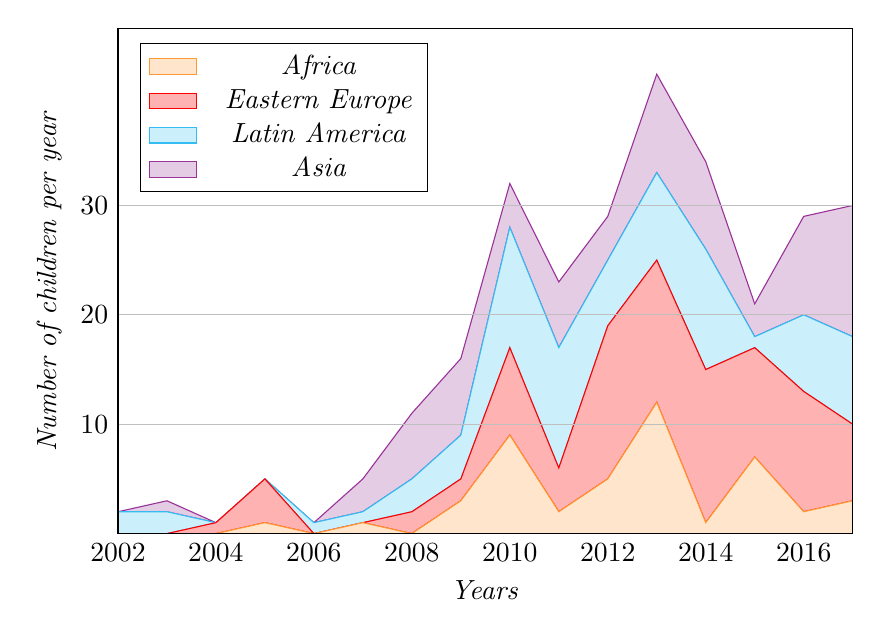
\begin{tikzpicture}
	\begin{axis}[
		stack plots=y,
		area style,
		enlarge x limits=false,
		enlarge y limits=upper,
		width=0.9\textwidth,
		height=8cm,
		xlabel = \textit{Years},
         ylabel = \textit{Number of children per year},
         ytick = {10, 20, 30},
         ytick style={draw=none},
         xtick style={draw=none},
         x tick label style={/pgf/number format/.cd,%
          scaled x ticks = false,
          set thousands separator={},
          fixed},
         y tick label style={/pgf/number format/.cd,%
          scaled y ticks = false,
          set thousands separator={},
          fixed},
         ymajorgrids=true,
         legend style={column sep=8pt},
         legend pos = north west]
    \addplot [draw={orange!80!white},fill={orange!20!white}] coordinates %Africa
		{(2002, 0) (2003, 0) (2004, 0) (2005, 1) (2006, 0) (2007,1 ) (2008, 0) (2009, 3) (2010, 9) (2011, 2) (2012, 5) (2013, 12) (2014, 1) (2015, 7) (2016, 2) (2017, 3)} 
		\closedcycle;
		\label{figdata:africa}
	\addplot coordinates % Eastern Europe
		{(2002, 0) (2003, 0) (2004, 1) (2005, 4) (2006, 0) (2007, 0) (2008, 2) (2009, 2) (2010, 8) (2011, 4) (2012, 14) (2013, 13) (2014, 14) (2015, 10) (2016, 11) (2017, 7)} 
		\closedcycle;
		\label{figdata:easterneurope}
	\addplot [draw={cyan!80!white},fill={cyan!20!white}] coordinates % Latin America
		{(2002, 2) (2003, 2) (2004, 0) (2005, 0) (2006, 1) (2007, 1) (2008, 3) (2009, 4) (2010, 11) (2011, 11) (2012, 6) (2013, 8) (2014, 11) (2015, 1) (2016, 7) (2017, 8)} 
		\closedcycle;
		\label{figdata:latinamerica}
		\addplot [draw={violet!80!white},fill={violet!20!white}] coordinates  % Asia
		{(2002, 0) (2003, 1) (2004, 0) (2005, 0) (2006, 0) (2007, 3) (2008, 6) (2009, 7) (2010, 4) (2011, 6) (2012, 4) (2013, 9) (2014, 8) (2015, 3) (2016, 9) (2017, 12)} 
		\closedcycle;
		\label{figdata:asia}
		\legend{\textit{Africa},\textit{Eastern Europe},\textit{Latin America},\textit{Asia}}
	\end{axis}
\end{tikzpicture}
\caption{Our population distribution - Total of children visited via the screening protocol, stratified by geographic area of origin}
\label{fig:populationperyear}
\end{figure}

\subsection{Inclusion and exclusion citeria}\label{sub:inclusionandexclusionciteria}
Lorem ipsum dolor sit amet, consectetur adipiscing elit. Pellentesque nibh metus, suscipit a scelerisque sit amet, rhoncus et lectus. Mauris eget erat rutrum, euismod massa id, maximus mauris. Nulla maximus, ex sit amet lacinia consequat, enim ante mollis dui, sit amet tincidunt massa felis id magna. Aenean gravida ante nec volutpat rutrum. Cras eget ullamcorper leo. Curabitur eu volutpat tellus. Integer nec ornare sapien. Fusce ipsum justo, interdum quis libero a, mattis tristique velit. Phasellus rhoncus lorem non ultrices luctus.

%QUI CHI È DENTRO E CHI È FUORI E PERCHÉ. ELENCO PUNTATO?

\section{The data set}\label{sec:dataset}
Lorem ipsum dolor sit amet, consectetur adipiscing elit. Pellentesque nibh metus, suscipit a scelerisque sit amet, rhoncus et lectus. Mauris eget erat rutrum, euismod massa id, maximus mauris. Nulla maximus, ex sit amet lacinia consequat, enim ante mollis dui, sit amet tincidunt massa felis id magna. Aenean gravida ante nec volutpat rutrum. Cras eget ullamcorper leo. Curabitur eu volutpat tellus. Integer nec ornare sapien. Fusce ipsum justo, interdum quis libero a, mattis tristique velit. Phasellus rhoncus lorem non ultrices luctus.

%QUI SPIEGHI COME SONO STATI RACCOLTI I DATI DA COLONNA
%E' stato usato Microsot Excel
% RIFERISCI A tab:columnparameter O INSERISCILA QUI

\section{Data set elaboration}\label{sec:datasetelaboration}
Lorem ipsum dolor sit amet, consectetur adipiscing elit. Pellentesque nibh metus, suscipit a scelerisque sit amet, rhoncus et lectus. Mauris eget erat rutrum, euismod massa id, maximus mauris. Nulla maximus, ex sit amet lacinia consequat, enim ante mollis dui, sit amet tincidunt massa felis id magna. Aenean gravida ante nec volutpat rutrum. Cras eget ullamcorper leo. Curabitur eu volutpat tellus. Integer nec ornare sapien. Fusce ipsum justo, interdum quis libero a, mattis tristique velit. Phasellus rhoncus lorem non ultrices luctus.

%QUI SPIEGHI COME E' FATTO IL DB

\subsection{VBA expressions}\label{sub:vbaexpressions}
Lorem ipsum dolor sit amet, consectetur adipiscing elit. Pellentesque nibh metus, suscipit a scelerisque sit amet, rhoncus et lectus. Mauris eget erat rutrum, euismod massa id, maximus mauris. Nulla maximus, ex sit amet lacinia consequat, enim ante mollis dui, sit amet tincidunt massa felis id magna. Aenean gravida ante nec volutpat rutrum. Cras eget ullamcorper leo. Curabitur eu volutpat tellus. Integer nec ornare sapien. Fusce ipsum justo, interdum quis libero a, mattis tristique velit. Phasellus rhoncus lorem non ultrices luctus.

All VBA expression can be found in Appendix \ref{chap:appendixvbaexpressions} at page \pageref{chap:appendixvbaexpressions}.

\subsection{Cut-off values}\label{sub:cutoffvalues}
Cut-off values for these results were established via the most recent literature review.

%INSERT WHERE THEY COME FROM
%INSERT TABLES HERE

\subsubsection{Haemoglobin}\label{sub:haemoglobin}
This was a little prick, but we managed with \cite{Hbcutoff} (from WHO).
It depends on:
\begin{enumerate}
	\item Sex
	\item Age
	\item Altitude (looking only at sea level)
\end{enumerate}
Based on Haemoglobin levels, we stratified anemias in:
\begin{enumerate}
	\item Non-Anemia
	\item Mild
	\item Moderate
	\item Severe
\end{enumerate}
This is summarized in Table that follows.

%INSERT ELENCO PUNTATO DA COSA DIPENDE
%INSERT TABLE HERE
%OCCHIO ALLE UNITÀ DI MISURA!
%Fai riferimento all'Appendice corrispondente.

\subsubsection{MCV}\label{sub:mcv}
This was ANOTHER little prick, but we managed with \cite{MCVferritincutoff}. It depends on various factors:

\begin{enumerate}
	\item Sex
	\item Age
	\item \dots
\end{enumerate}

%INSERT ELENCO PUNTATO DA COSA DIPENDE
%INSERT TABLE HERE
%OCCHIO ALLE UNITÀ DI MISURA!
%Fai riferimento all'Appendice corrispondente.

\subsubsection{Circulating Iron}\label{sub:iron}
This was easy.

%INSERT WHAT IT MEANS
%INSERT TABLE HERE
%OCCHIO ALLE UNITÀ DI MISURA!
%Fai riferimento all'Appendice corrispondente.

\subsubsection{Vitamin D}\label{sub:vitaminD}
Vitamin D is healthy. We dosed $25\-OH$ or \textit{colecalciferol} (1,25(OH)2D: 1,25-dihydroxyvitamin D and 25(OH)D: 25-hydroxyvitamin D)...\\
Recent literature has openly discussed about how vitamin D deficiency should be defined, especially in pediatric age. \cite{vitDcutoff1} is a really strong and recent (2018) Italian review on vitamin D deficiency. Another review is in \cite{vitDcutoff2}. From BMJ is \cite{vitDcutoff3}. And maybe strongest of all the letter addressed to BMJ from the British Society of Pediatric Radiology and child protection and nutrition committees of the Royal College of Pediatrics and Child Health in \cite{vitDcutoff_letter}.\\
General international consensus is on defining cut-off values based on alkaline phosfatase and calcium levels so to enhance ONLY bone health, ignoring the now well-known vitamin D extra-skeletal effects.

As explained in \ref{sec:roleofpediatrician}, internationally adopted children often suffer from vitamin D deficiency or insufficiency, because of the profound change in latitude they experience during the adoption phase, or because of malnutrition combined with lack of solar exposure during pre-adoptive care, usually in orphanages.

%INSERT WHAT IT MEANS
%https://en.wikipedia.org/wiki/Calcifediol
%INSERT WHY THIS HAS BEEN DOSED
%INSERT TABLE HERE with ng/dL and nanomol/L (o quel che è)
%OCCHIO ALLE UNITÀ DI MISURA!
%Fai riferimento all'Appendice corrispondente.

\subsection{Parasites grouping}\label{sub:parasites}
These are the considered pathogens.

\begin{itemize}
	\item Group 1
		\begin{enumerate}
			\item Entamoeba
			\item Ancylostoma
			\item Trichuris
		\end{enumerate}
	\item Group 2
		\begin{enumerate}
			\item Giardia
			\item Strongyloides
			\item Hymenolepis
			\item Blastocystis
			\item Endolimax
		\end{enumerate}
\end{itemize}

We conceived them like this:

\begin{itemize}
	\item Group 1: Parasites responsible for gastrointestinal bleeding and, therefore, iron-deficient mycroctic anemia .
	\item Group 2: Parasites responsible for gastrointestinal malabsorbtion.
\end{itemize}

%QUI SI PARLA DI PERCHE LI HAI DIVISI IN DUE GRUPPI E COME (SUL FATTO CHE FOSSERO ANEMIZZANTI O MENO) E POI VEDIAMO I RISULTATI
% IN \cite{GNLBIexp} C'è una tabella con cui comparare i risultati!!
%Fai riferimento all'Appendice corrispondente.

\section{Statistical Analyses}\label{sec:statisticalanalyses}
The descriptive analyses were conducted using frequencies and percentage for categorical variables, and means and standard deviations or medians and inter-quartile intervals for continuous ones. We preferred to use the latter because the scarcity of data prevented us from checking for normality.\\
Non parametrical tests, such as Mann-Whitney or Kruskal-Wallis tests, were employed to evaluate the difference in value of continuous variables in different groups. One test or the other was used based on the number of groups, case by case: if two, the Mann-Whitney test was used, if more than two, Krusal-Wallis. To study the relation between two dichotomous variables, or one dichotomous and one categorical, we used the two-tailed Fisher's exact test. To study whether a dichotomous event was associated to one or more independent variables, we used logistic regression.\\
In order to study the relation between continuous variables, we preferred using Spearman's rank correlation.

All statistical analyses were conducted using the Stata/IC software, version 14.2 (StataCorp LLC, College Station, USA).
%DA RILEGGERE %TODO

%Testo originale
%Le analisi descrittive sono state condotte utilizzando frequenze e percentuali per variabili categoriche, e medie e deviazioni standard o mediane e intervalli interquartili per variabili continue, con una preferenza per queste ultime a causa del campione esiguo di dati che non consente di verificare la normalità dei dati.
%La differenza nei valori di variabili continue in diversi gruppi è stata valutata con test non parametrici di Mann-Whitney o Kruskal-Wallis a seconda che i gruppi da confrontare fossero due o più di due. Per lo studio di associazione tra due variabili dicotomiche, o tra una variabile dicotomica e una categoriale ordinata abbiamo utilizzato il test esatto di Fisher a due code. Per studiare se un esito dicotomico fosse associato a una o più variabili indipendenti abbiamo utilizzato la regressione logistica.
%Per studiare la relazione tra due variabili continue, abbiamo preferito utilizzare la correlazione per ranghi di Spearman.
%Per tutte le analisi abbiamo usato il software Stata/IC 14.2 (StataCorp LLC, College Station, USA).

%RIFERMIENTI ALL'APPENDIX
% \cite{sec:ageinyears} \cite{asec:geographicarea} \cite{asec:pathologicalvalues} \cite{asub:patweightandheight} \cite{asub:pathaemoglobin} \cite{asub:patmcv} \cite{asub:patiron} \cite{asub:patferritin} \cite{asub:patvitaminD} \cite{asec:parasiticinfections} \cite{asub:parasitespos} \cite{asub:parasitegrouping}